%Fiquemos com Deus e Nossa Senhora!
%Sao Jose de Cupertino rogai por nos!!
% ### Uses XeLaTeX ### %
% ### Needs beamer-master ### %
\documentclass[aspectratio=169]{beamer} %. Aspect Ratio 16:9

\usetheme{AI2} % beamerthemeSprace.sty
\usepackage[portuguese]{babel}
\usepackage[utf8]{inputenc}
\usepackage[T1]{fontenc}
\usepackage{ragged2e,gensymb}

\DeclareMathOperator*{\argmin}{arg\,min}
\DeclareMathOperator*{\argmax}{arg\,max}
\DeclareMathOperator{\sign}{sgn}

% DATA FOR FOOTER
\date{2021}
\title{- Graph Neural Networks}
\author{João Paulo Papa}
\institute{Advanced Institute for Artificial Intelligence (AI2)}

\begin{document}
% ####################################
% FIRST SLIDE 						:: \SliTit{This is the Title of the Talk}{A. B. Name}{Sprace}
% SUB-TITLE SLIDE 					:: \SliSubTit{<title>}{<explanation}
% SUB-SUB-TITLE SLIDE				:: \SliSubSubTit{<title>}{<explanation}
% SLIDE WITH TITLE 					:: \SliT{Title}{Content}
% SLIDE NO TITLE 						:: \Sli{Content} 
% SLIDE DOUBLE COLUMN WITH TITLE 	:: \SliDT{Title}{First Column}{Second Column}
% SLIDE DOUBLE COLUMN NO TITLE 		:: \SliD{First Column}{Second Column}
% SLIDE ADVANCED WITH TITLE 			:: \SliAdvT{Title}{Content}
% SLIDE ADVANCED NO TITLE 			:: \SliAdv{Content}
% SLIDE ADVANCED DOUBLE WITH TITLE 	:: \SliAdvDT{Title}{First Column}{Second Column}
% SLIDE ADVANCED DOUBLE NO TITLE 	:: \SliAdvD{First Column}{Second Column}
% SLIDE BLACK						:: \Black{ <Content> }
% SLIDE WHITE						:: \White{ <Content> }
% ITEMIZATION 						:: \begin{itemize}  \iOn{First} \iTw {Second} \iTh{Third} \end{itemize}
% COMMENT TEXT				 		:: \note{<comment>}
% SECTION 							:: \secx{Section} | \secxx{Sub-Section}
% BOLD SPRACE COLOR				:: \bfs{<text>}
% TABLE OF CONTENT					:: \tocitem{<title>}{<content>}
% LEFT ALIGN EQUATION				:: \begin{flalign*}  & <equation> &   \end{flalign*}
% CENTER ALIGN EQUATION	S			:: \begin{gather*} <equations>  \end{gather*}
% SLASH								:: \slashed{<>}
% BAR								:: \barr{<letter>} instead of \bar{<letter>}
% THEREFORE						:: use \portanto (larger and bold}
% 2 or 3 MATH SYMBOLS				:: \overset{<up>}{<down>} &  \underset{<below>}{\overset{<above>}{<middle>}}  
% INSERT TEXT IN FORMULA			:: \ins{<text>}
% EXERCISE							:: \exe{<exercise #>}{<exercise text>}
% SUGGESTED READING BOX			:: \sug{<references>}
% CITATION							:: \cittex{<citation>}
% CITATION DOUBLE COLUMN 			:: \cittexD{<citation>}
% TEXT POSITION						:: \texpos{<Xcm>}{<Ycm>}{<text>} origin = center of slide : x right | y down
% REFERENCE AT BOTTOM  S/D SLIDE		:: \refbotS{<reference>} \refbotD{<reference>}
% HIDDEN SLIDE						:: \hid
% COLOR BOX 						:: \blu{blue} + \red{rec} + \yel{yellow} + \gre{green} + \bege{beige}
% FRAME 							:: \fra{sprace} \frab{blue} \frar{red} + \fray{yellow} + \frag{green}		
% FIGURE 							:: \img{X}{Y}{<scale>}{Figure.png} 
% FIGURE							:: \includegraphics[scale=<scale>]{Figures/.png}
% FIGURE DOUBLE SLIDE NO TITLE		::  \img{-4}{0.5}{<scale>}{Figure.png} % Image 1st half
%									::  \img{4}{0.5}{<scale>}{Figure.png} % Image 2nd half
% FIGURE DOUBLE SLIDE WITH TITLE		::  \img{-4}{0}{<scale>}{Figure.png} % Image 1st half
%									::  \img{4}{0}{<scale>}{Figure.png} % Image 2nd half
% INCLUDING SWF (Flash)				:: \usepackage{media9} and \includemedia >> USE ACROBAT <<
%%%%%%%%%%%%%%%%%%%%%%%%%%%%%%%%%%%%%%%%%%%%%%%%%%
% ###############################################################################
% FIRST SLIDE
\SliTit{{\LARGE Graph Neural Networks}}{Advanced Institute for Artificial Intelligence -- AI2}{https://advancedinstitute.ai}
%%%%%%%%%%%%%%%%%%%%%%%%%%%%%%%%%%%%%%%%%%%%%%%%%%
% ###############################################################################
% SLIDE SUB-TITLE
%\SliSubTit{Sub-Title}{Description}{}
%%%%%%%%%%%%%%%%%%%%%%%%%%%%%%%%%%%%%%%%%%%%%%%%%%
% ###############################################################################
%\SliSubSubTit{Sub-Sub-Title}{Description}
 %%%%%%%%%%%%%%%%%%%%%%%%%%%%%%%%%%%%%%%%%%%%%%%%%%


\SliT{Introdução}{

\justifying Sabemos que um grafo pode ser definido como ${\cal G} = ({\cal V},{\cal E})$, em que ${\cal V}$ e ${\cal E}$ correspondem ao conjunto de \textbf{vértices} (ou nós) e \textbf{arestas}, respectivamente. Grafos podem ser utilizados para modelar diversas entidades, tais como imagens, textos, interações entre usuários em redes sociais e moléculas, por exemplo.\newline

\justifying Tarefas de predição em grafos podem ser efetuadas em três níveis:

\begin{itemize}
	\item Grafo: a tarefa é a de predizer as propriedades do grafo propriamente dito (ex: qual o tipo de molécula que estamos analisando?).
	\item Vértice: a tarefa é a predizer o papel de cada nó no grafo (ex: classificação de um determinado usuário em uma rede social).
	\item Arestas: a tarefa é a de predizer a ação representada por uma determinada aresta (ex: classificação de ações em imagens).
\end{itemize}
}

\Sli{
\justifying \emph{Graph Neural Networks} (GNNs) podem ser entendidas como uma transformação otimizável em todos os atributos do grafo (nós, arestas e o grafo propriamente dito) que \textbf{preserva as suas simetrias} (invariâncias à permutações). De maneira geral, podemos usar diferentes informações para cada nível de atuação de uma GNN:

\begin{itemize}
	\item Grafo: número de nós, caminho mais longo, valor calculado na MST (\emph{Minimum Spanning Tree}), etc.
	\item Vértice: número de vizinhos, peso do nó, etc.
	\item Arestas: peso da aresta, etc.
\end{itemize}
}

\Sli{
\justifying Usualmente, uma GNN emprega uma rede MLP (\emph{Multilayer Perceptron}) em cada componente do grafo, dando origem ao que chamamos de \textbf{camada GNN}.

\begin{center}
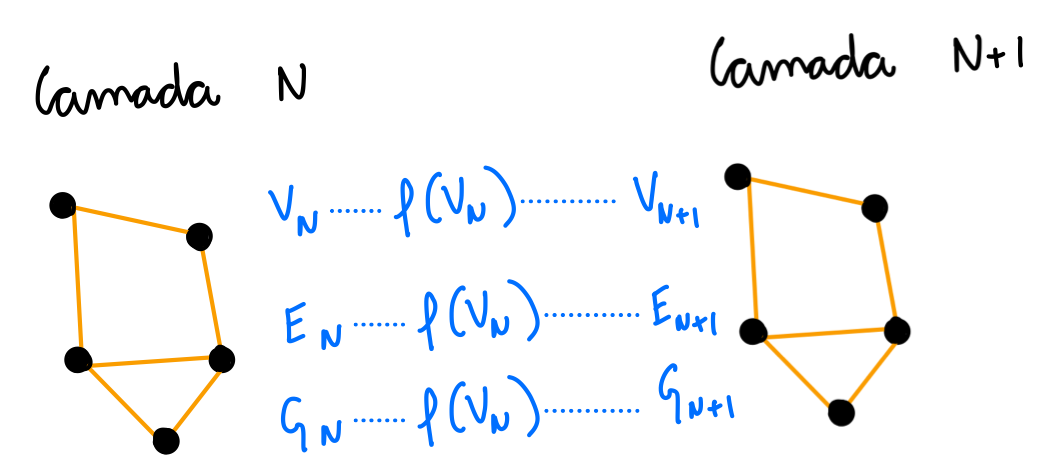
\includegraphics[scale=0.2]{./figs/GNN_Fig1.png}
\end{center}

\justifying Assim, temos que $f(\cdot)$ é a função (MLP) que recebe como entrada uma entidade (grafo, vértice ou aresta) e retorna algum tipo de processamento sobre ele. Note, portanto, que uma GNN não atualiza a conectividade do grafo, representada pela sua lista de adjacências.
}

\Sli{
\justifying Dado que temos uma GNN, como podemos utilizá-la para fazer predições? Vamos considerar um caso de \textbf{classificação binária}. Caso a tarefa seja a de realizar predições nos nós e eles já possuem alguma informação (\emph{node embedding}), basta aplicarmos um classificador em cada um deles para obter a predição.

\begin{center}
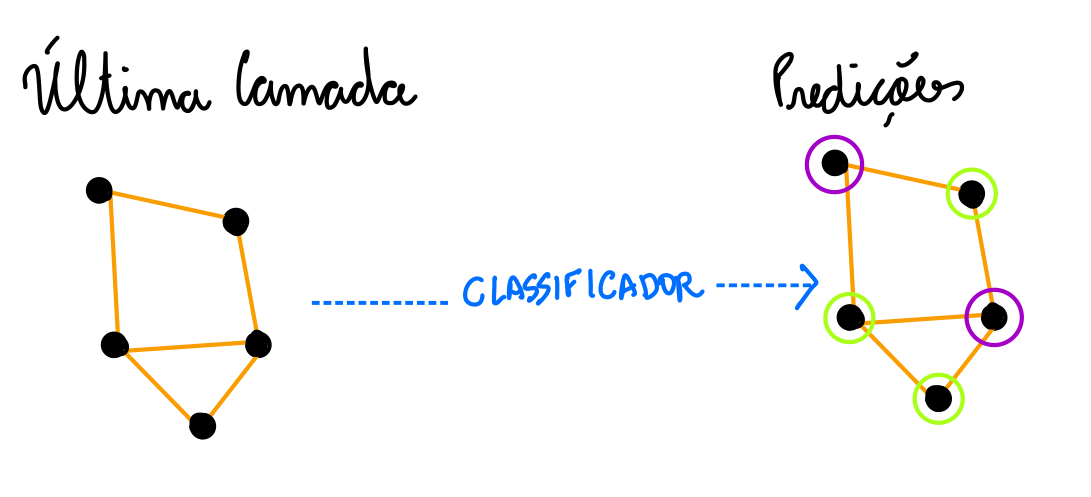
\includegraphics[scale=0.2]{./figs/GNN_Fig2.png}
\end{center}

\justifying No entanto, podemos enfrentar situações mais complicadas como, por exemplo, ter informações nas arestas mas ainda querer realizar predições nos nós. Assim, precisamos de uma maneira para coletar informações das arestas e passá-las aos nós para fins de predição.
}

\Sli{
\justifying Podemos realizar tal etapa por meio de uma operação de \emph{pooling}. Podemos realizar isto em duas etapas:

\begin{itemize}
	\item Para cada entidade (aresta) que iremos aplicar o \emph{pooling}, podemos criar uma matriz concatenando suas informações (embeddings). Ex: para um nó com duas arestas adjacentes, suas respectivas informações serão agrupadas.
	\item Agregar as informações (usualmente uma operação de soma é aplicada à todas elas).
\end{itemize}
Podemos representar a operação de pooling pela letra $\rho$ e denotar que estamos juntando (passando) informações de arestas para os nós da seguinte maneira: $\rho_{{\cal E}_N\rightarrow {\cal V}_N}$, em que $N$ representa a camada em questão que a operação está sendo realizada.
}

\Sli{
\justifying  Assim sendo, caso tenhamos apenas informações sobre arestas e queiramos realizar predições nos nós, podemos utilizar \emph{pooling} para passar (rotear) informações para serem utilizadas posteriormente.

\begin{center}
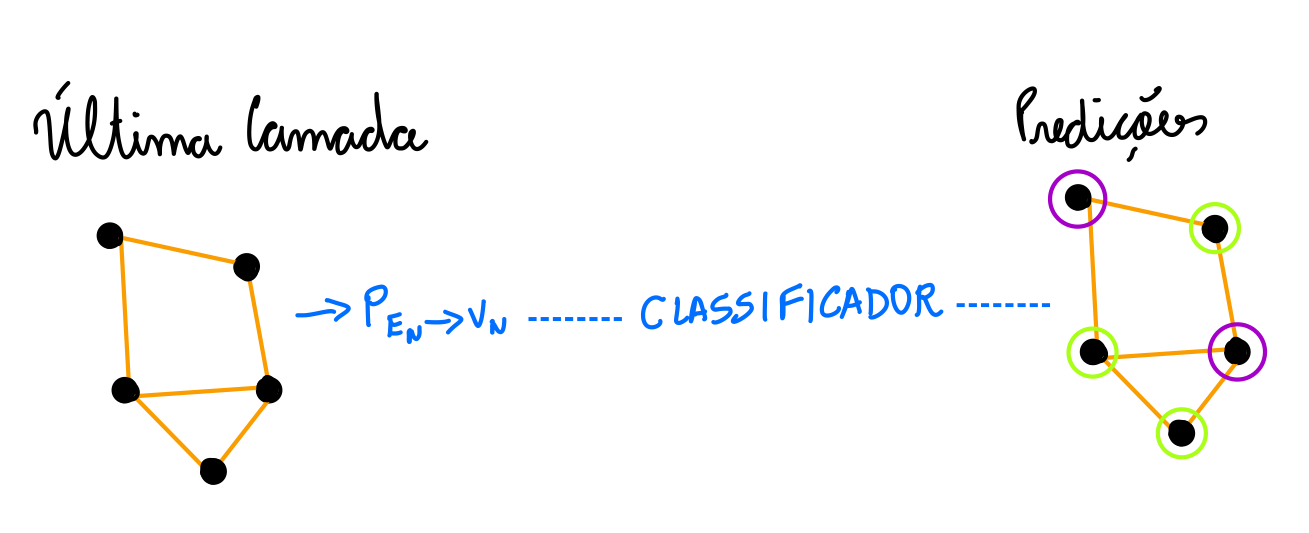
\includegraphics[scale=0.2]{./figs/GNN_Fig3.png}
\end{center}
}

\Sli{
\justifying Por outro lado, caso tenhamos apenas informações sobre os nós e queiramos realizar predições nas arestas, podemos realizar algo semelhante.

\begin{center}
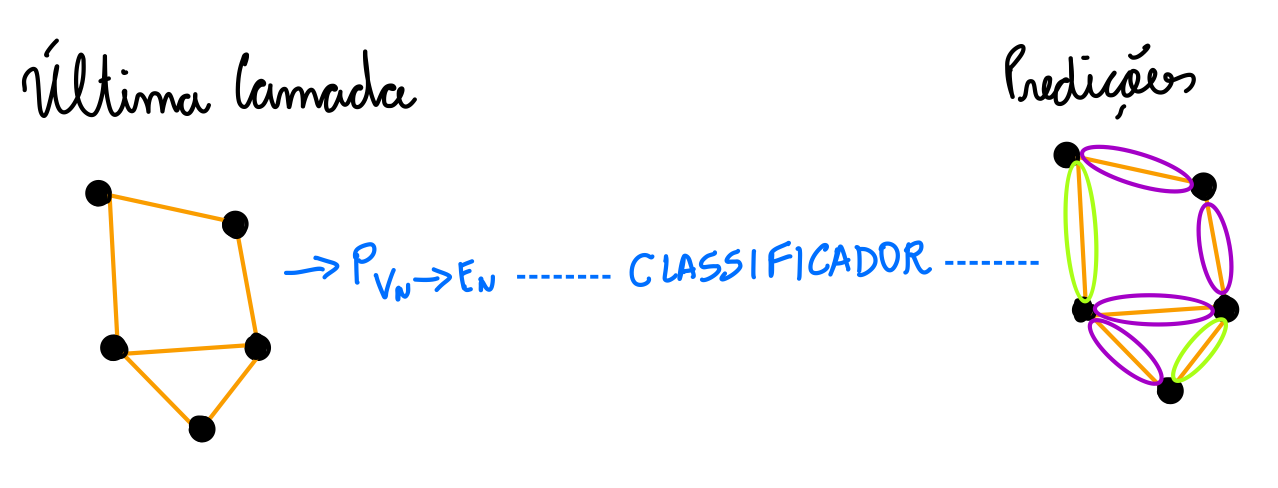
\includegraphics[scale=0.2]{./figs/GNN_Fig4.png}
\end{center}
}

\end{document}